\section{Introduction}
\label{sec:introduction}

Multidimensional indexes are vital components in database systems that store
large amounts of high-dimensional data. In high-dimensional databases data 
analysis is often based on range search or nearest neighbor search queries. 
Multidimensional index structures can benefit such queries, by restricting
search to smaller areas.

Figure~\ref{fig:fcluster} shows an example of the multidimensional search
problem on the \texttt{Employees} table. The \texttt{Employees} table consists
of five attributes, i.e., the employee id, the monthly salary, the years
of experience, the age of each employee and the department each employee 
belongs to.
A database administrator (DBA) has identified a set of columns,
from the \texttt{Employees} relation where a
multidimensional clustering should be considered
\footnote{We assume the presence of a DBA for simplicity, although we 
will discuss other options later on the paper.}. For instance, consider
 columns age, salary and years of experience as the ones chosen by the DBA
to be clustered. Now consider a query of the following form.

\begin{flushleft}
\texttt{\textsc{select} age, salary, experience\\
\textsc{from} Employees\\
\textsc{where} age > 26 \textsc{and} age $\leq$ 30 \textsc{and}\\
salary > 22 \textsc{and}  salary $\leq$ 49 \textsc{and}\\
experience > 4 \textsc{and} experience $\leq$ 8}
\end{flushleft}

\begin{flushleft}
\texttt{\textsc{select} age, salary, experience\\
\textsc{from} Employees\\
\textsc{where} age > 24 \textsc{and} age $\leq$ 28 \textsc{and}\\
salary > 21 \textsc{and}  salary $\leq$ 56 \textsc{and}\\
experience > 2 \textsc{and} experience $\leq$ 7}
\end{flushleft}

\begin{figure}[t]
\begin{center}
\vspace*{3\baselineskip}
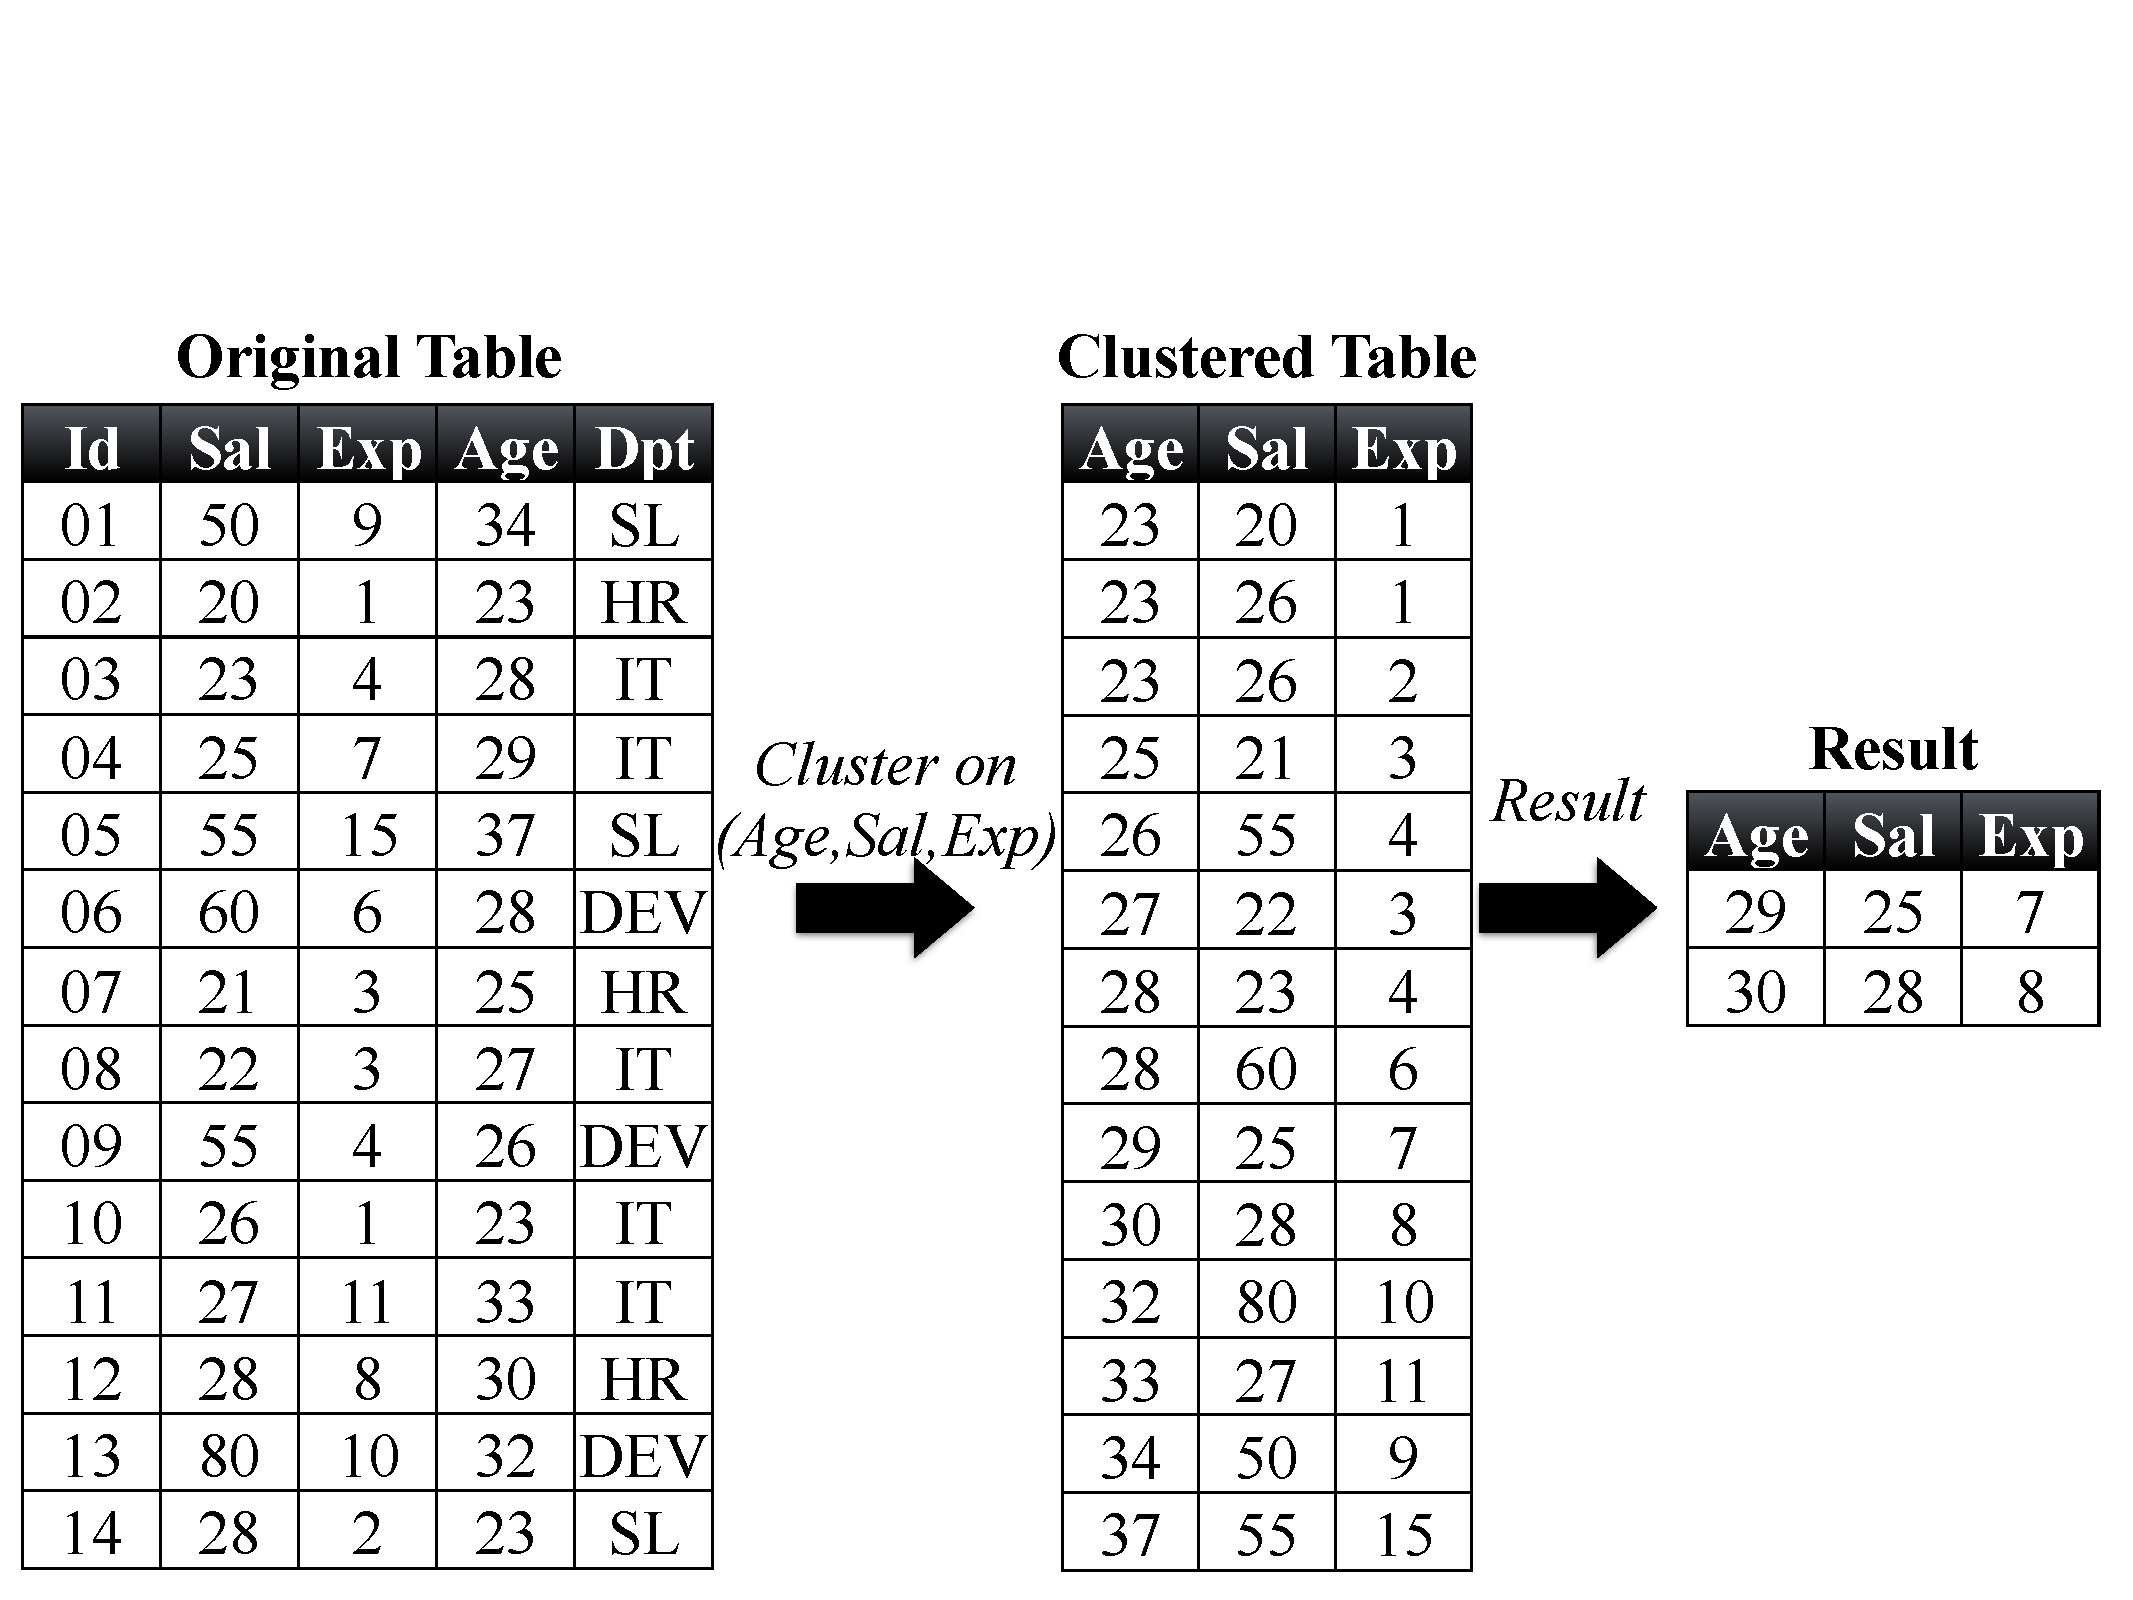
\includegraphics[trim=0cm 2cm 0cm 9.5cm, width=\columnwidth]{Figures/example_relation}
\caption{Multidimensional search on fully clustered data.}
\label{fig:fcluster}
\end{center}
\end{figure}

Ideally, to answer every query of this form we would like to have all the
relevant columns clustered as shown in Figure~\ref{fig:fcluster}.
On top of the clustered data we would use a structure to navigate directly
to the qualifying tuples. However, clustering is based on sorting, and thus,
it is a very expensive process.
Furthermore, clustering all data would delay the processing of the first query
if we did not have 
enough time to finish clustering before. To avoid penalizing user queries
with the big clustering overhead, we can \emph{partially} cluster the data.
A multidimensional index is used then to navigate search queries to clusters
with candidate qualifying tuples as shown in Figure~\ref{fig:pcluster}.
Finally, we scan the list of candidates
in order to find the tuples that qualify all predicates. 

\begin{figure}[t]
\begin{center}
\vspace*{3\baselineskip}
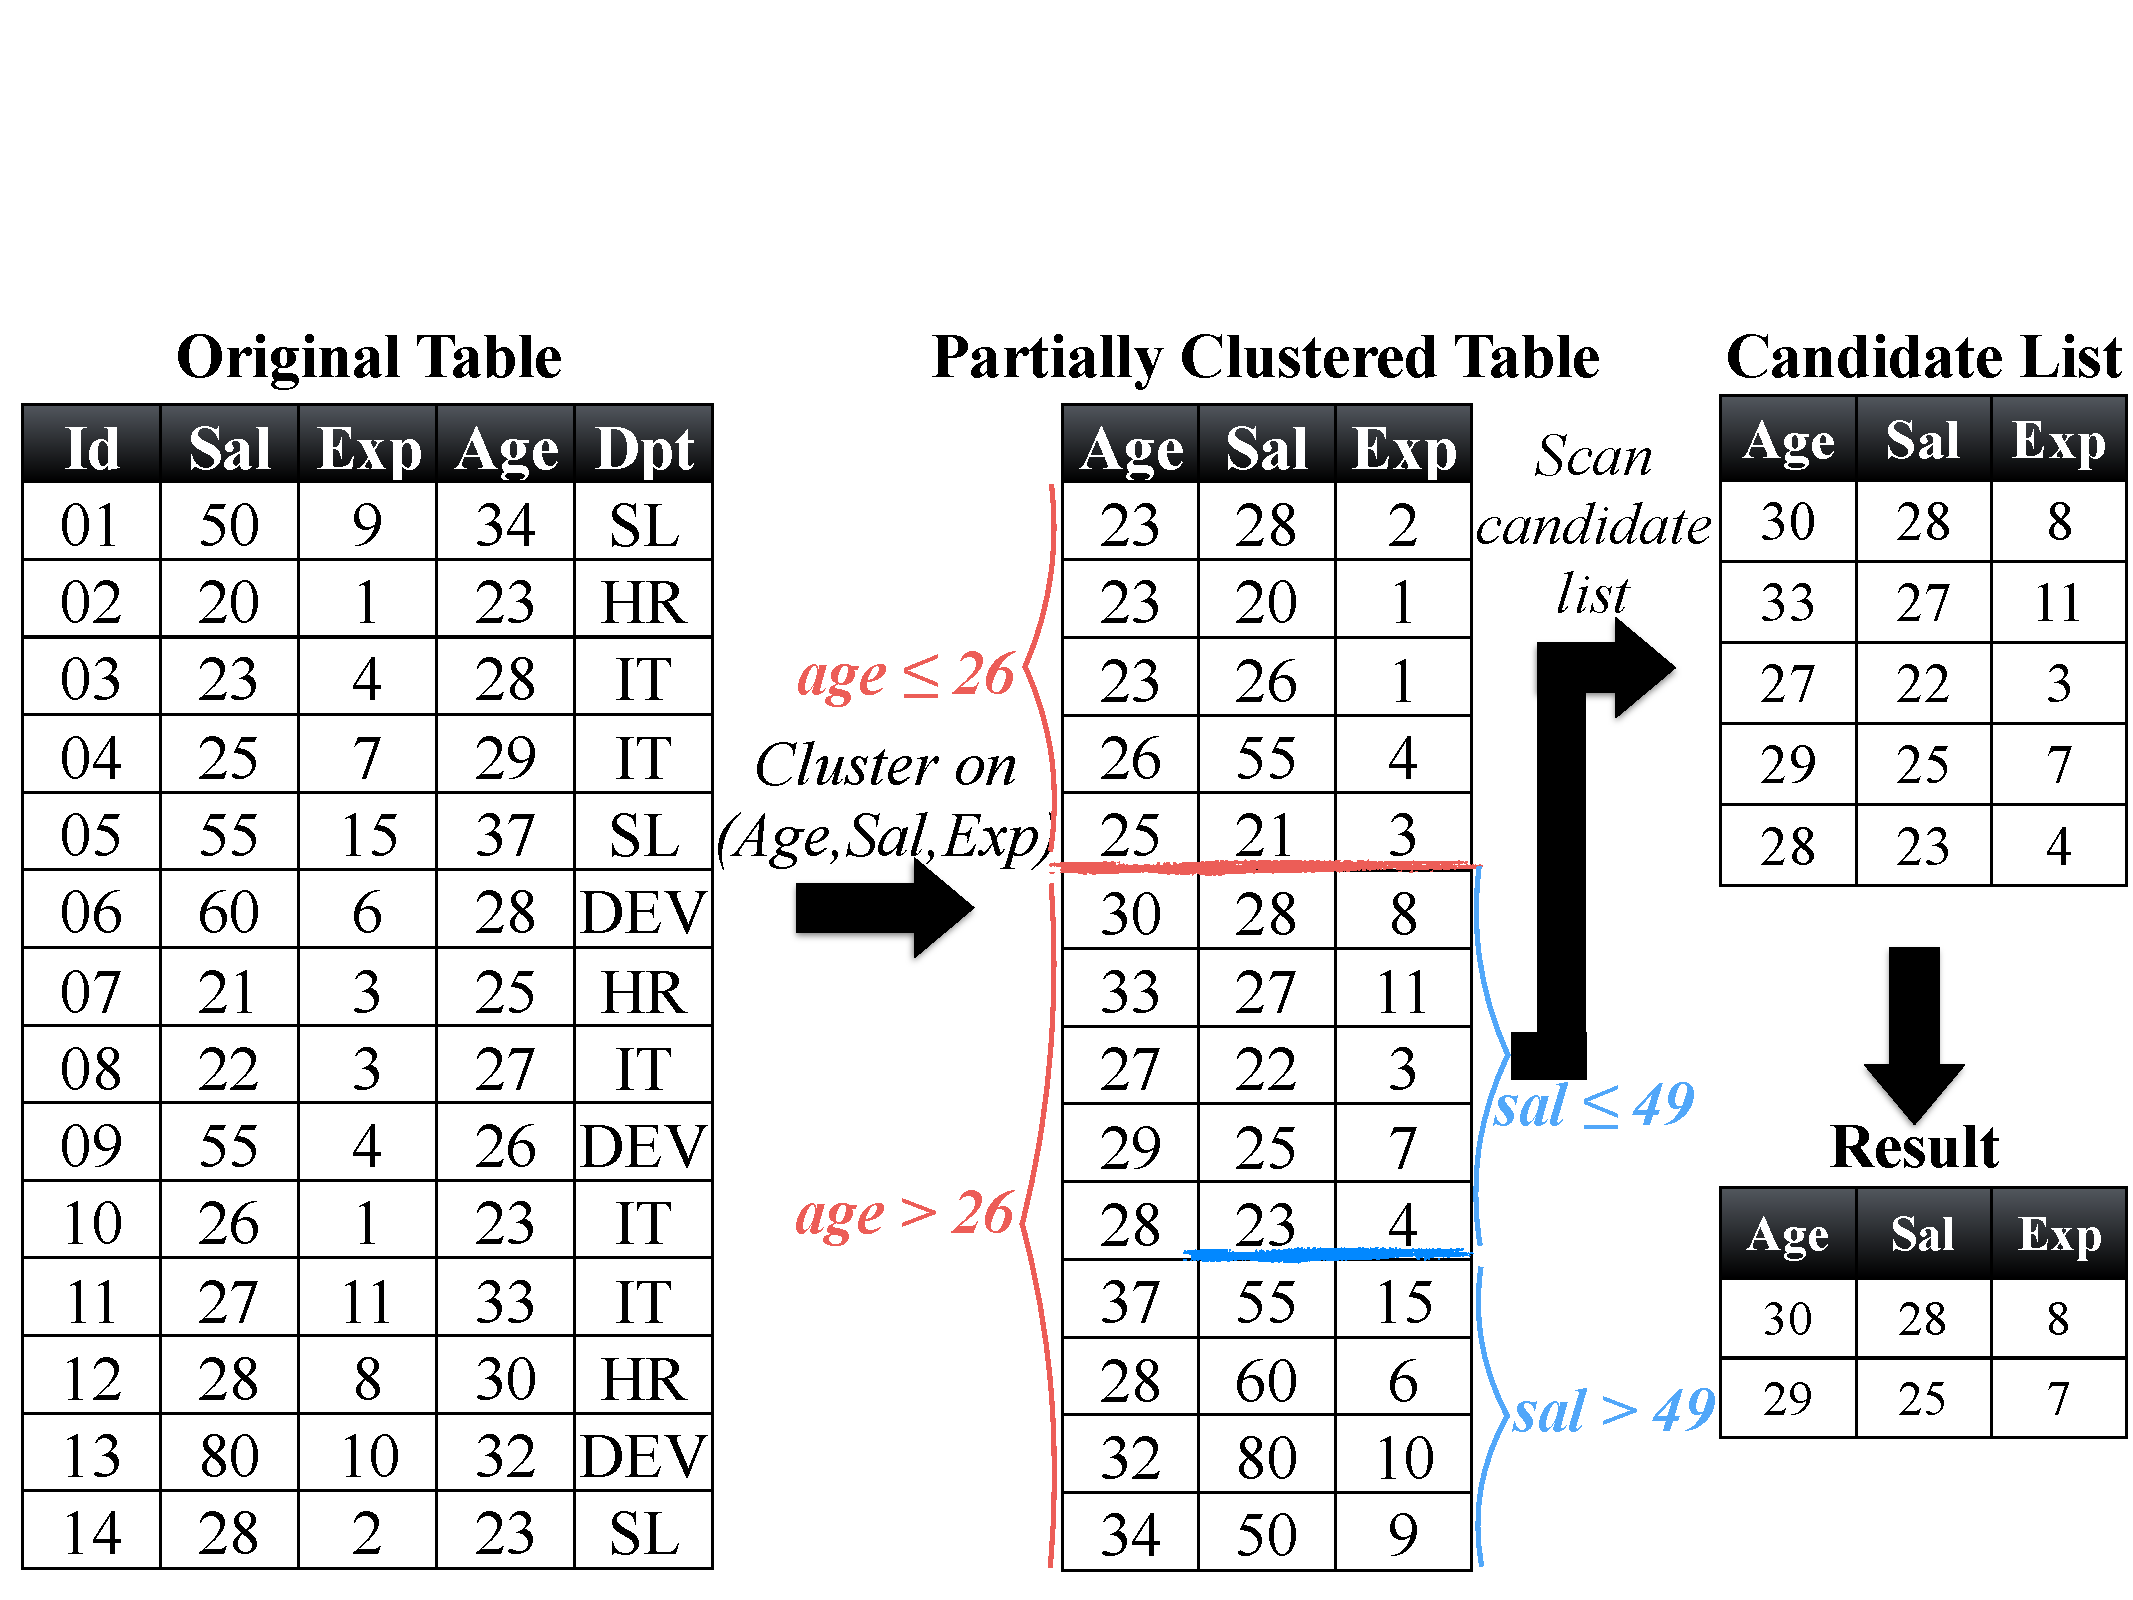
\includegraphics[trim=0cm 2cm 0cm 8.5cm, width=\columnwidth]{Figures/mcrack_relation}
\caption{Multidimensional search on partially clustered data.}
\label{fig:pcluster}
\end{center}
\end{figure}

Partial clustering is driven by the query predicates. For example, 
in Figure~\ref{fig:pcluster}, we first create two clusters based on the age
of the employees. Employees that are younger than 26 years belong to
the first cluster, while employees that are older than 26 years belong
to the second cluster. Similarly, the second crack, clusters the employees
that are older than 26 years into two new clusters; the first one that
contains employees that receive a monthly salary less than 50 hundred and
the second one that contains employees that receive more than 50 hundred per
month. After the two cracks, we have a list of candidate tuples,
which contains employees that are older than 26 with a monthly salary
less than 50 hundred. Out of the candidate list, we need to identify finally
those employees that are younger than 31 years, get a monthly salary
greater than 24 hundred and have an experience between 4 and 9 years.

In order to store the clustering information and to navigate to 
clusters with candidate tuples, we need a multidimensional index
structure, like a $kd$-tree. The $kd$-tree stores query predicates 
along with the cracking position in the nodes. Figure~\ref{fig:pkdtree}
shows the contents of the $kd$-tree after each crack in the previous
query. Later, we will
explain in detail how the $kd$-tree structure is adjusted to our
needs and we will provide the necessary definitions.

\textbf{Adaptive Multidimensional Indexing.}
We propose an adaptive indexing solution which minimizes the index 
creation time allowing users to query the data soon after its generation
and several times faster compared to state-of-the-art indexing approaches.  
As more queries are processed, the index is continuously refined and
subsequent queries enjoy better execution times. 
The concept of adaptive indexing has been studied in the context
of a single dimension in column-oriented databases.
In uni-dimensional cracking the main goal is to incrementally sort
individual arrays (i.e., columns) for point or range queries.
In this paper we extend the adaptive indexing idea to apply on multiple
dimensions. To  simultaneously index multiple attributes,
we need to introduce different techniques than unidimensional cracking.

\textbf{Contributions.} Our contributions are summarized as follows.
\begin{itemize}
  \setlength{\itemsep}{0pt}
  \setlength{\parskip}{0pt}
  \setlength{\parsep}{0pt}
\item We demonstrate the inability of state-of-the-art indexing to cope with exploratory analysis of very large multi-dimensional data collections. We show that the index creation time is a major bottleneck which becomes worse as data grows.
\item We introduce a novel adaptive clustering technique.  Adaptive clustering minimizes the data to query gap by integrating indexing actions with query processing and being able to immediately process user queries.
The index structure is continuously enriched as more data and queries arrive and only for the hot part of the data.
\item Furthermore,  we  propose adaptive clustering algorithms that automatically expand hot subtrees in the hot branches of the index to minimize querying costs.
\item Through a detailed experimental evaluation with both synthetic and diverse real-world workloads, we show that it is possible to drastically reduce the data to query time, being able to handle thousands of queries by the time that state-of-the-art multidimensional indexing (KDTree \cite{DBLP:journals/cacm/Bentley75}) techniques are still in the index creation phase.
\end{itemize}

\textbf{Paper outline.}
The rest of the paper is organized as follows.
In Section~\ref{sec:related_work} we discuss existing multidimensional index structures.
Section~\ref{sec:background} provides the necessary background for database cracking.
Section~\ref{sec:adaptive_partitioning} describes multidimensional adaptive indexing 
providing necessary definitions and discussions over the adaptive index built process 
and the multidimensional index structure we use.
Section~\ref{sec:experiments} describes a thorough experimental analysis with both 
real and synthetic workloads.
Finally, Section~\ref{sec:conclusions} concludes the paper.

